\FloatBarrier
\section{Validation and Experimental Protocols}
\label{sec:experiments-appendix}

\FloatBarrier
\subsection{Arithmetic and Implementation Validation}
\label{sec:experimental-validation}

The successful Lean 4.24.0 build and axiom audit cover 64 local declarations,
including the exponential remainder, finite signed tensor contractions,
full-score block enclosure, and composed real-attention quotient. The only
axioms are \texttt{propext}, \texttt{Classical.choice}, and \texttt{Quot.sound};
\artifact{results/lean-verification.json}{Lean audit manifest} records source hashes and per-theorem
dependencies. The polygon optimizer, rational exponential routine, BF16 cell
constructor, state identity, and CUDA instruction semantics remain separate
implementation obligations.

The 46-test CPU suite includes randomized enclosure tests, 500 exact polygon
comparisons with an independent half-plane intersection implementation,
40 direct 100-digit attention comparisons across rank and refinement, and
40 numerical/exact geometry comparisons. Invalid dimensions, nonintegral
indices, negative bounds, unsupported domains, stale source/query/shift state,
and midpoint behavior are covered.

\begin{samepage}
This audit found an arithmetic defect:
integer endpoints allowed reciprocal evaluation through Python's floating-point
\mbox{\texttt{1 / int}}, so the upper endpoint of $[1,1]/[3,3]$ could lie below $1/3$.
Endpoints and scale factors now normalize to exact fractions; the regression
requires both endpoints to equal $1/3$ exactly.
\end{samepage}

The imported CUDA checker retains all 74 rational-certified rows among
160 rationally generated rows, certifies no rationally refused row in that
fixture, and rejects 13 invalid-domain or strict-boundary controls. Numerical
fixtures compare the original, shared-scalar, and parallel implementations and
dense block correction against CPU results. Memory, race, and synchronization
checks report no errors on the exercised numerical paths; imported CUDA memory
checking also reports no errors. These finite checks complement the theorem
chain without establishing instruction-level correctness for all inputs.

\FloatBarrier
\subsection{Exact-Rational Coupling Checks}
\label{sec:coupling-validation}

Independent high-precision coverage comparisons use 110 decimal digits and a
scaled $10^{-95}$ tolerance to compare against exact zero-width intervals.
An initial zero-tolerance attempt failed through cancellation in a constant
channel and is documented. Certificate and rational-oracle comparisons use
exact fractions without this tolerance. Stored decimal endpoints are display
approximations; broad-channel failures and exact-midpoint abstentions remain
in the artifact.

\begin{table}[!htbp]
  \centering
  \caption{Initial exact-rational coupling results. Denominators count
  coordinates, not independent model examples.}
  \label{tab:coupling-results}
  \begin{tabular}{lr}
    \toprule
    Result & Count \\
    \midrule
    Box certificate accepts & $57/149$ \\
    Coupled certificate accepts & $61/149$ \\
    Global hull accepts & $50/149$ \\
    Narrower coupled residual & $30/149$ \\
    Unchanged residual width & $119/149$ \\
    Accepts beyond global hull & $1$ \\
    False certificate / coverage failure & $0$ \\
    \bottomrule
  \end{tabular}
\end{table}

\FloatBarrier
\subsection{Uncertainty Localization and GPU Controls}
\label{sec:localized-uncertainty}

The CPU experiment in \cref{sec:coupling-experiment} isolates correction work.
\Cref{fig:selective-refinement} shows the selected token fractions for every
query before the GPU controls below compare complete-output coverage and cost.

\begin{figure}[!htbp]
  \centering
  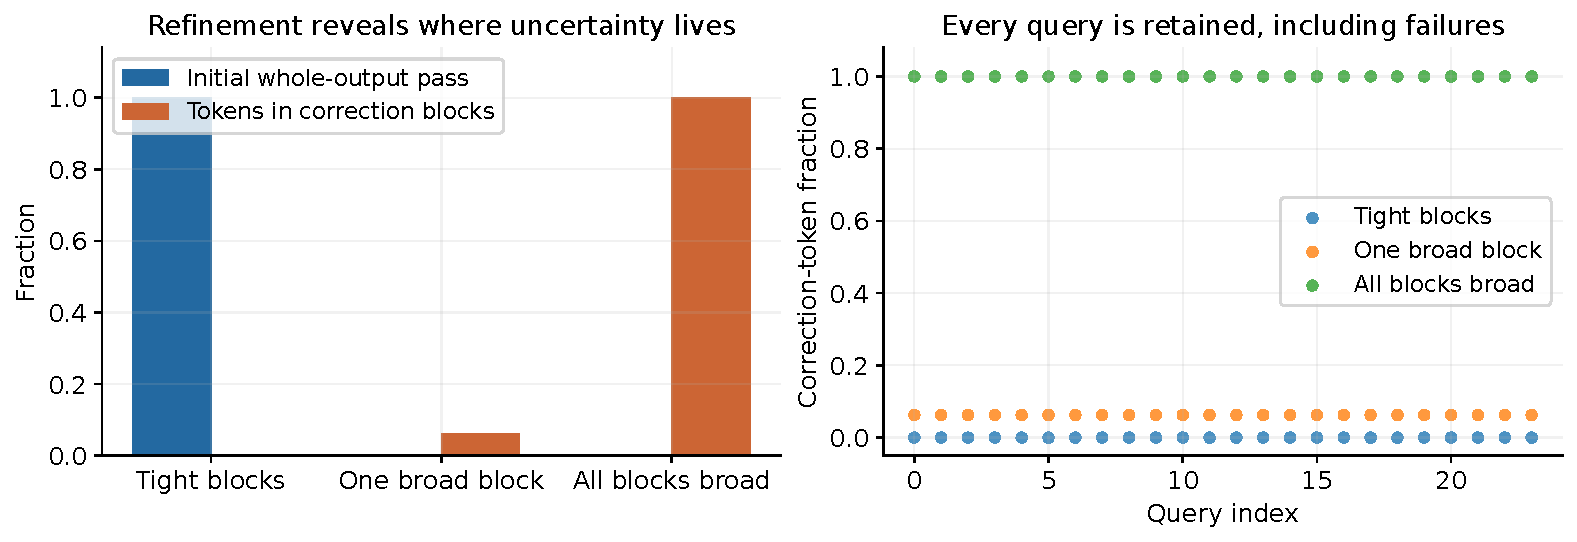
\includegraphics[width=\textwidth]{figures/selective_refinement.pdf}
  \caption{Correction-token fractions for every query in tight, mixed, and
  broad CPU inputs. Local uncertainty permits local correction; diffuse
  uncertainty requires all tokens. Full-source validation reads are additional
  and included in CPU timings.}
  \label{fig:selective-refinement}
\end{figure}

GPU synthetic controls use $d=h=64$ and BF16 input values represented exactly
in binary64 on the summary path. Tight clusters can pass completely. Moderate
cases pass 10,197 of 19,008 coordinates across configurations but none of
297 complete outputs; these aggregates reuse seeded inputs across ranks.
The centered-value control passes 1,986 of 2,048 coordinates but only 6 of
32 outputs. Complete-output acceptance is a conjunction of coordinate
decisions, so high marginal coverage need not yield useful output coverage.
This observation assumes no coordinate independence. Exact-midpoint controls
reject every strict cell by design. In the measured GPU path, one failed
coordinate triggers full-batch fallback (\cref{fig:gh200-coverage-cost}).

\begin{figure}[!htbp]
  \centering
  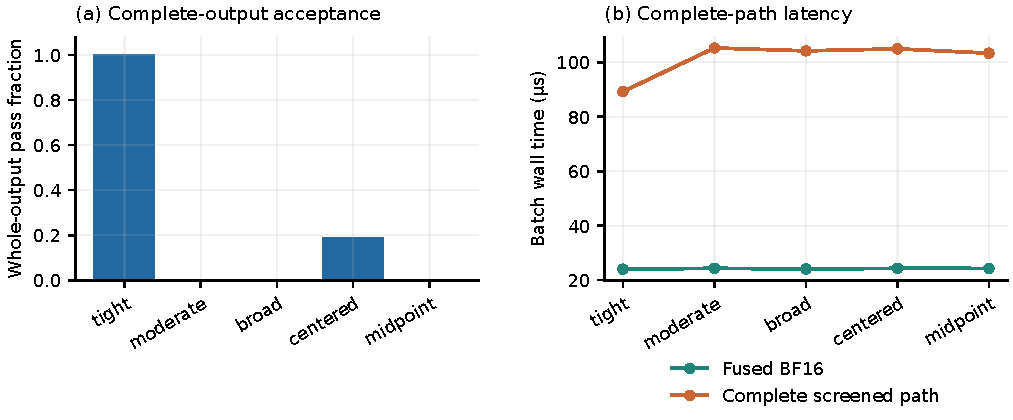
\includegraphics[width=\textwidth]{figures/gh200_coverage_cost.pdf}
  \caption{Whole-output coverage and complete GPU costs for rank-four,
  $N=8192$, $Q=32$ controls varying uncertainty and cell margins. The cost
  includes the full-batch fallback triggered by any failed coordinate.}
  \label{fig:gh200-coverage-cost}
\end{figure}

\FloatBarrier
\subsection{Trained-Activation Capture and Diagnostics}
\label{sec:trained-protocol}

No coordinate or whole output passes the numerical screen on either trained
activation set. Rank eight covers all 24 layers and 14 query heads over six
prefixes: 2,016 head instances and 129,024 coordinates. Full rank covers layers
0, 12, and 23, adding 252 head instances. We capture actual post-RoPE Q/K/V
arguments at the attention call of Qwen2.5-0.5B \citep{qwen25}, pinned revision
\texttt{060db64} (the full commit hash is recorded in the
\artifact{results/model_traces/manifest.json}{capture manifest}), using
Transformers 4.51.3
and BF16 weights. Three deterministic original texts cover prose, code, and
arithmetic at prefix lengths 1,024 and 4,096. The final prefill query sees the
entire prefix; contiguous GQA groups contain seven query heads per KV head,
and scaling by $1/8$ is exact. This is an activation diagnostic, not a
language-model accuracy benchmark or production-traffic sample.

\begin{table}[!htbp]
  \centering
  \caption{Medians of trained-activation radius and cell-margin diagnostics.
  Full rank uses the three representative layers.}
  \label{tab:trained-radii}
  \begin{tabular}{lrr}
    \toprule
    Diagnostic & Rank 8 & Rank 64 \\
    \midrule
    Maximum-block retained bound $\rho$ & 1.32 & 29.91 \\
    Maximum-block discarded bound $\epsilon$ & 34.24 & 0 \\
    Actual maximum projected score deviation & 0.85 & 8.91 \\
    Minimum-channel BF16 boundary margin
      & $8.95\times10^{-7}$ & $6.66\times10^{-7}$ \\
    \bottomrule
  \end{tabular}
\end{table}

\begin{figure}[!htbp]
  \centering
  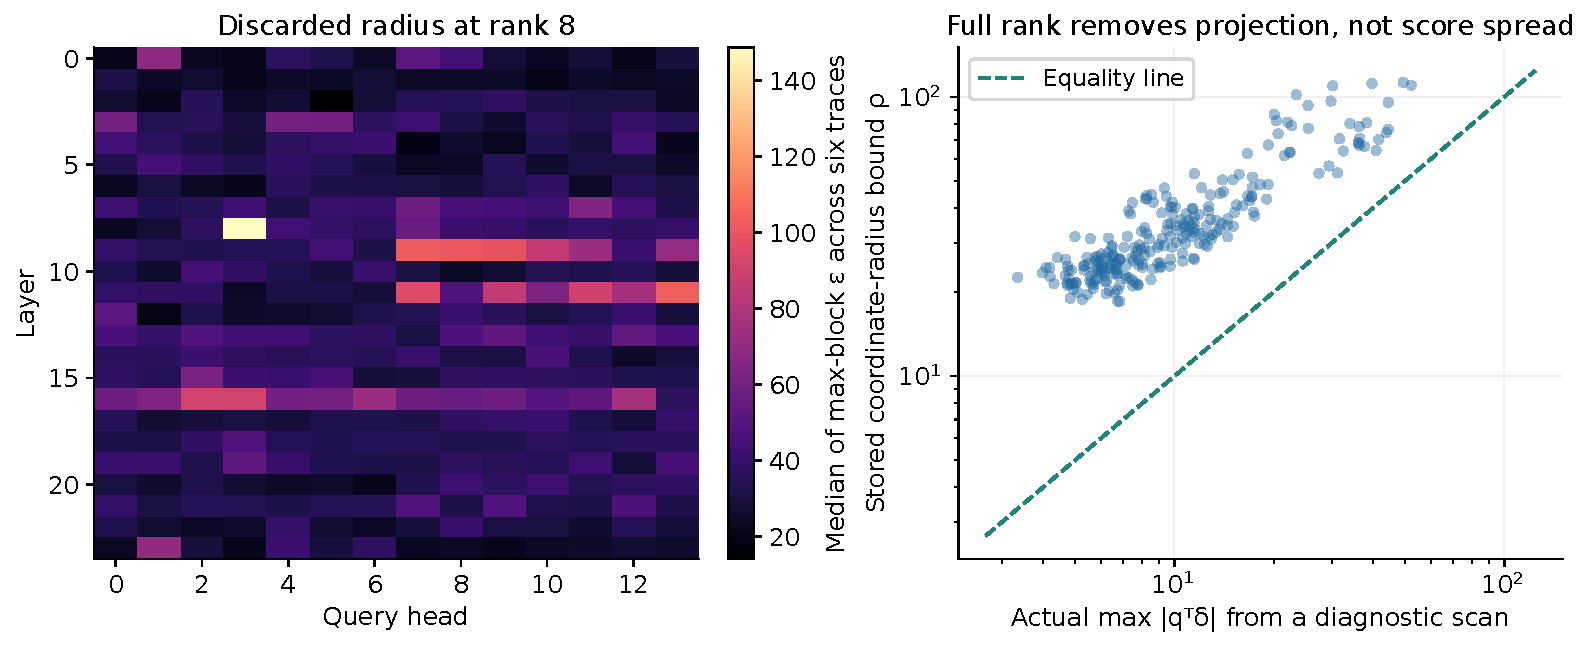
\includegraphics[width=\textwidth]{figures/model_score_radii.pdf}
  \caption{Trained-model score radii by layer and head. Low rank leaves large
  discarded-score variation; full-rank coordinate bounds exceed scan-derived
  radii, while actual score variation remains substantial. Computing scanned
  diagnostic radii reads tokens and is not free query metadata.}
  \label{fig:model-score-radii}
\end{figure}

\FloatBarrier
\subsection{GH200 Environment and Timing Protocol}
\label{sec:gh200-protocol}

The final sweep contains 57 synthetic and nine actual prose trace/rank
configurations on one NVIDIA GH200: compute capability 9.0, 97,871 MiB reported
GPU memory, driver 580.105.08, CUDA 12.8, and PyTorch 2.7.0. Synthetic cases vary
$N\in\{1024,8192,32768\}$, rank, spread, and $Q\in\{1,32\}$. Here $Q=32$
is a noncausal query batch sharing K/V, not independent serving requests.
Trace cases use seven query heads sharing one KV head at the final prefix.

The baseline explicitly forces PyTorch's fused FlashAttention SDPA backend
\citep{flashattention}, matching BF16 input values, scale, visible keys, and
zero dropout. A separate binary64 softmax/matmul computation checks outputs.
Seven samples of 20 invocations provide raw CUDA-event and host-wall times;
plotted quantiles summarize those samples, not workload confidence intervals.
Resident timings exclude setup; construction, uploads, casts, allocations,
workspace, and graph capture are recorded separately. Complete eager timings
include screening, device decision reduction, CPU synchronization, and either
an output cast or executed full-batch fallback (\cref{fig:gh200-latency}).

\begin{figure}[!htbp]
  \centering
  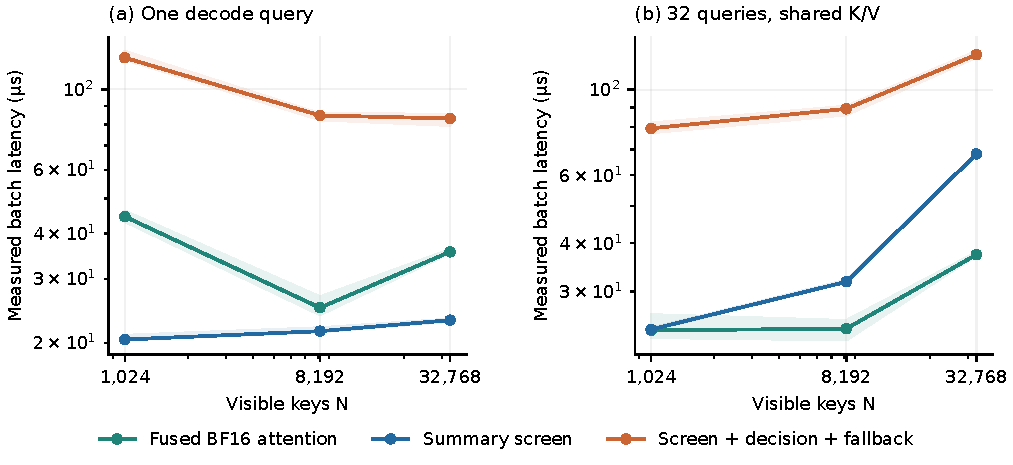
\includegraphics[width=\textwidth]{figures/gh200_latency.pdf}
  \caption{GH200 resident screening and complete-path latency against fused
  dense attention for tight rank-four inputs. Wall-clock medians and
  10th--90th sample quantiles include each complete path's actual decisions
  and fallback behavior.}
  \label{fig:gh200-latency}
\end{figure}

The eager timing helper performs three warmup calls and synchronizes before
sampling. Each sample brackets 20 invocations with CUDA events, waits for the
ending event, and divides both event elapsed time and host-wall elapsed time
by 20. Host samples therefore include Python launch and synchronization
costs. Graph measurements first warm the operation on a separate stream,
capture 20 invocations with fixed inputs, then warm graph replay three times
and collect seven replay samples. Reported replay times are divided by 20;
graph capture time is stored separately. No adaptive scheduler or fallback is
captured in the replay graph.

All 66 recorded cases use seed 902105. The 57 synthetic configurations contain
19 tight, 18 moderate, 18 broad, one centered-value, and one exact-midpoint
case. Seeded input generation is repeated across retained ranks, so aggregate
acceptance counts reuse inputs. The nine GPU trace cases are three prose
captures, from layers 0, 12, and 23 at prefix length 4,096, evaluated at ranks
0, 4, and 16. They are separate from the rank-eight and full-rank CPU activation
diagnostics.

\FloatBarrier
\subsection{Kernel Ablation, Setup, and Footprint}
\label{sec:gh200-costs}

Even the favorable $N=32768,Q=1,r=4$ case loses end to end. Its resident
parallel screen takes \SI{20.09}{\micro\second} under fixed-input graph replay
versus dense attention's \SI{31.30}{\micro\second}; the complete eager path
takes \SI{83.11}{\micro\second} versus \SI{35.62}{\micro\second}, plus about
\SI{51.50}{\milli\second} of reusable summary/workspace setup. CPU
moment-and-extrema arrays occupy 1,000,448 bytes, the uploaded box summary
869,376 bytes, and original BF16 K/V 8,388,608 bytes. These payloads exclude
262,144 bytes of group indices and Python object/hash overhead; scratch and
retained original K/V are reported separately. Neither serving-system memory
savings nor a complete-path speedup follows. Every measured complete path is
slower than dense, so no finite reuse count repays setup under these costs
(\cref{fig:gh200-amortization}).

\begin{table}[!htbp]
  \centering
  \caption{Matched graph replay medians in microseconds for tight rank-four
  inputs. All three screening implementations and the dense baseline are
  retained, including the adverse small-input case.}
  \label{tab:gh200-ablation}
  \begin{tabular}{rrrrrr}
    \toprule
    $N$ & $Q$ & Original & Shared scalar & Parallel & Dense \\
    \midrule
    1024 & 32 & 20.47 & 19.87 & 20.84 & 9.80 \\
    8192 & 1 & 35.69 & 35.60 & 18.72 & 14.55 \\
    32768 & 1 & 118.65 & 118.14 & 20.09 & 31.30 \\
    32768 & 32 & 143.28 & 147.52 & 64.89 & 34.21 \\
    \bottomrule
  \end{tabular}
\end{table}

\begin{figure}[H]
  \centering
  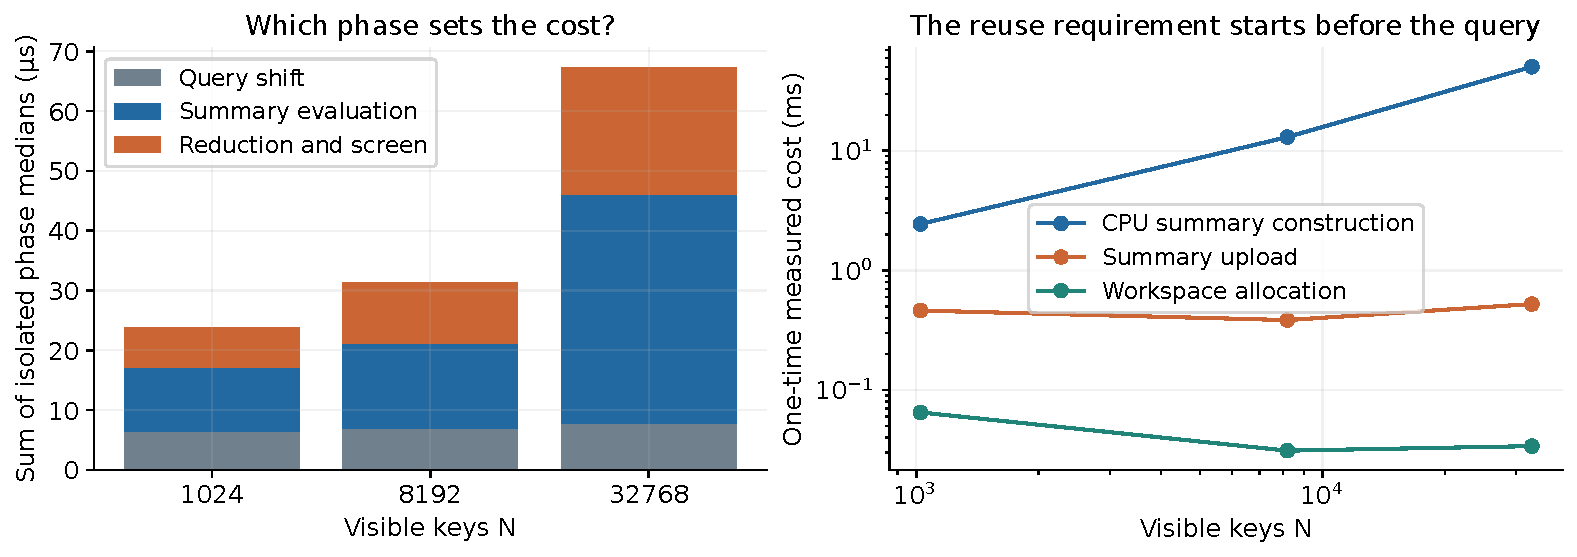
\includegraphics[width=\textwidth]{figures/gh200_cost_breakdown.pdf}
  \caption{Isolated GPU phase medians and summary setup costs. CPU
  construction, upload, and workspace allocation remain explicit; complete
  latency is measured separately rather than reconstructed from phase sums.}
  \label{fig:gh200-cost-breakdown}
\end{figure}

\begin{figure}[H]
  \centering
  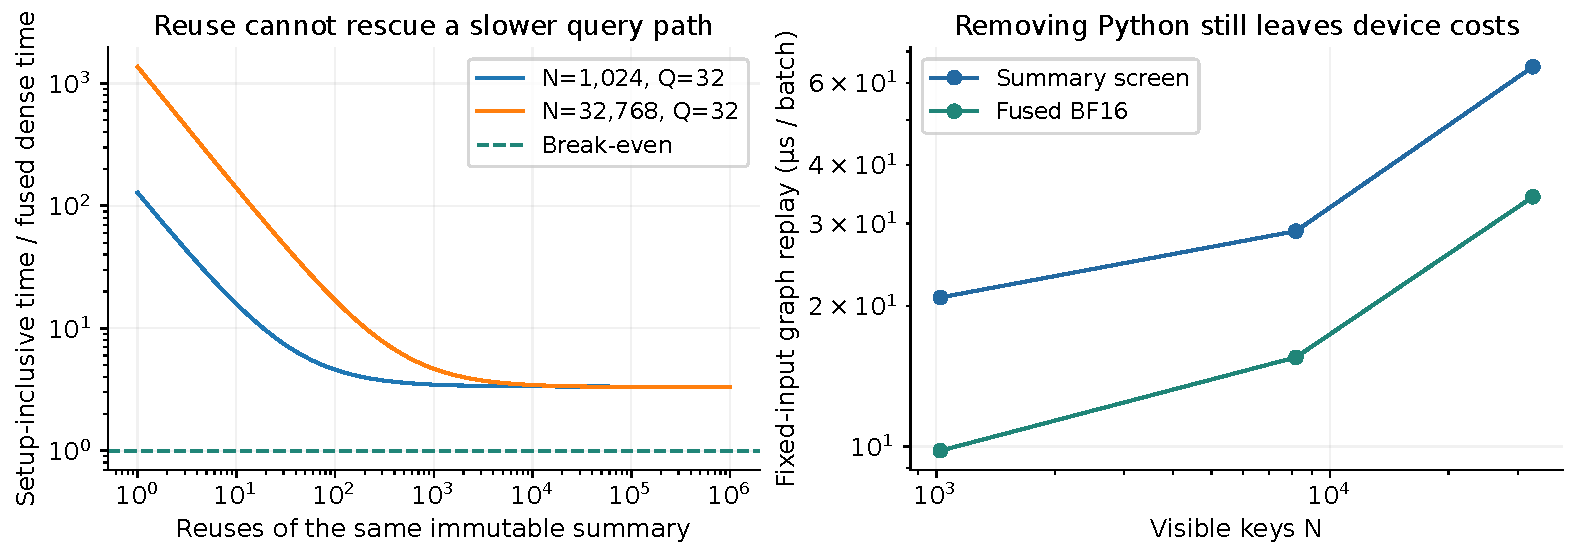
\includegraphics[width=\textwidth]{figures/gh200_amortization.pdf}
  \caption{Setup amortization and matched graph device costs. No measured
  complete path has a finite setup break-even. Fixed-input graph replay omits
  the adaptive host decision and constitutes a separate experiment.}
  \label{fig:gh200-amortization}
\end{figure}

\begin{minipage}{\textwidth}
\subsection{Retained Failures and Same-Machine Reproduction}
\label{sec:gh200-reproduction}

The first trained-trace parity attempt failed nine absolute-residual tolerance
checks because broad bounds had extremely large magnitudes. A scaled
$10^{-12}$ comparison addresses this diagnostic scaling while still requiring
identical screen decisions and independent output checks; the maximum observed
scaled variant difference is $1.33\times10^{-15}$. The nine failures and original
scalar-only sweep are preserved. This tolerance changes implementation-parity
diagnostics, not certificate bounds.

Figures and tables retain the first complete sweep. A second GH200 run measures
commit \texttt{d2c3668}, including final host ABI guards and formatted sources.
\artifact{results/gh200/provenance.json}{GH200 provenance manifest} records source, library, and trace hashes;
both original and reproduction measurements remain available. All 66 cases
pass validation again with unchanged coverage and mismatch counts. Parallel
screen graph medians change by $-1.08\%$ to $+1.42\%$ across cases, with median
ratio $1.002$. Complete-path and dense host-wall medians are noisier, with
median ratios $1.075$ and $1.112$. Every complete screened path remains slower
than dense, with no finite setup break-even. This reproduces the conclusions
on the same machine, without estimating variation across devices, model
families, or serving systems.
\par
\end{minipage}

\FloatBarrier
